\fancyhf{}
\pagestyle{fancy}
%Encabezado
\lhead[]{\leftmark}
\chead[]{}
\rhead[]{\thepage}
\renewcommand{\headrulewidth}{1pt}

El correspondiente trabajo final de Licenciatura en Ciencias de la Computación, en los tres primeros capítulos se explicaron conceptos relacionados a la temática de Comprensión de Programas (CP) y Análisis de Identificadores (ids). El estudio de estos temas tiene como objetivo ubicar al lector en el contexto de estas temáticas y además brindar un estado de arte acorde a las mismas. 
A partir del estudio del estado del arte de las técnicas de análisis de ids, se detectó que no todas estas técnicas están implementadas en herramientas automáticas. Una herramienta con tales características facilita entender el propósito de los ids en los códigos. Cuando una persona ajena a un código de software, entiende con facilidad el significado de los ids, comprende mejor el sistema de estudio \cite{EZH08,DFPM05,BCPT00,DMDJ13}, por ende la construcción de esta herramienta es un aporte directo al área de la CP. Teniendo en cuenta esta ausencia de implementaciones, se llevó a cabo el desarrollo de una herramienta que a través de una interfaz amigable, le ayuda al usuario a analizar los ids presentes en los códigos. Esta herramienta llamada IDA, fue descripta en el capítulo anterior y a través de distintos casos de estudios, se explayó el aporte que hace al área de la CP. Para concluir con este trabajo final, en este último capítulo se describen algunos aspectos generales sobre IDA, se brindan algunas conclusiones y se proponen trabajos futuros a realizar.

\section{Herramienta Identifier Analizer (IDA)} 

En este apartado, se describen características generales de la herramienta IDA que servirán de introducción para detallar distintas propuestas relacionadas a trabajos futuros.

La herramienta IDA (Identifier Analizer) consta de tres módulos, el primero consiste en un Analizador Sintáctico, el segundo de dos algoritmos de división (Greedy, Samurai) y el tercero de un algoritmo de expansión básico, en los próximos párrafos se explican características de cada uno de ellos:

\begin{description}

\item[Analizador Sintáctico (AS):] Permite extraer con facilidad los elementos estáticos presentes en los códigos escritos en JAVA. Estos elementos son, los ids como objetos principales, los comentarios y los literales. Luego toda esta información capturada, se almacena en estructuras internas de IDA para que esté disponible en próximos módulos y se presente en tablas para que el usuario pueda visualizarla.

\end{description}

Finalizada la captura de los elementos por medio del AS, en el próximo módulo, IDA le permite al usuario escoger entre dos técnicas de división de ids, que se describen a continuación:

\begin{description}

\item[Algoritmo Greedy:] Esta técnica utiliza un diccionario con palabras en Inglés (proveniente de ispell\footnote[1]{ http://wordlist.aspell.net}), un listado de abreviaciones conocidas y una lista de palabras reservadas. El algoritmo realiza la división del id cuando algún substring del mismo es encontrado en algunos de estos diccionarios/listas.
Para lograrlo, lo primero que realiza el algoritmo es dividir al id tomando como referencia las marcas de separación entre dos palabras (si existen). Ejemplo: el guión bajo \textsf{in\_put} $\rightarrow$ \textsf{in put}, o camel-case \textsf{inPut} $\rightarrow$ \textsf{in put} (hardwords). El resto de las palabras resultantes (softwords), se someten a un proceso recursivo de división.
Este proceso, se lleva a cabo con dos rutinas una denominada \textbf{buscarPrefijo} y la otra \textbf{buscarSufijo}, la primera busca el prefijo más largo posible y la segunda el sufijo más largo posible. Ambas búsquedas (de prefijos y sufijos) consisten en ir consultando los diccionarios/listas descriptas al principio del párrafo. Una vez que las rutinas encuentran un prefijo o sufijo en el id, colocan una marca de división que lo separan del resto, luego las rutinas continúan con lo que quedan del id hasta que no haya más palabras que dividir. El resultado que más divisiones tenga entre las dos rutinas será seleccionado (ver capítulo 3 - sección \ref{sec:algGre}).

\item[Algoritmo Samurai:] Este algoritmo considera que las palabras que contiene un id multi-palabra se encuentran en algún sitio del código de estudio o en códigos de otros programas. La división del id estará determinada por la frecuencia de aparición de estas palabras. 
Samurai consulta la frecuencia de aparición de las palabras del código de estudio actual, a través de una tabla de frecuencias local. Por otro lado, Samurai obtiene la frecuencia de aparición de palabras obtenidas de una variedad de programas, por medio de una tabla de frecuencias global.
Estas tablas (local y global) predefinidas, son consultadas por la función de score, la misma recibe como entrada una palabra y retorna un puntaje que se determina de acuerdo a la frecuencias de aparición de cada palabra.
Samurai, al principio actúa de manera similar a la técnica Greedy, divide al id con espacios en blanco, en lugares donde se destaquen la división entre dos palabras (si existen), como el caso de guión bajo, camel-case, (hardwords).
Luego, las palabras resultantes (softwords), se procesan de manera recursiva de izquierda a derecha, buscando un punto de división entre dos partes. La función de score le dará un puntaje a cada parte, si son lo suficientemente altos se procederá a dividir entre ambas partes, sino continuará analizando el resto (ver capítulo 3 - sección \ref{sec:algSamu}).

\end{description}

Una vez que fueron divididos los ids, las distintas partes resultantes se someten a un proceso de expansión por medio de una técnica, que se explica a continuación:
\pagebreak
\begin{description}
\item[Algoritmo de Expansión Básica:] Este algoritmo se encarga de tomar palabras que resultaron producto de la separación de ids. En caso de que estas palabras estén abreviadas, el algoritmo de expansión las expande a su correspondiente palabra completa. Para lograrlo, se utilizan los comentarios o literales capturados del código por medio del AS, si los mismos son escasos, se recurre a un diccionario de palabras en Inglés como último recurso (ver capítulo 3 - sección \ref{sec:algExpBas}). Dado que este algoritmo no esta preparado para elegir una única expansión entre múltiples posibilidades, ante esta posibilidad se decidió implementar una elección aleatoria, de esta manera siempre se retornará un único resultado.

\end{description}

Los resultados conseguidos, producto de las técnicas descriptas anteriormente se muestran en tablas para que el usuario pueda visualizar y sacar conclusiones. Los casos de estudio del capítulo 4 mostraron que la división Samurai tiene mejor comportamiento que la Greedy, esto es lógico, debido que Greedy es un algoritmo muy primitivo \cite{DLFB06,FBL06,HDD06}. Con respecto a las expansiones, el algoritmo correspondiente, si bien también es sencillo y no cuenta con procesos complejos \cite{LFBEX07}, expande los ids de manera aceptable, de acuerdo a la información que captura el AS por medio de los comentarios y literales.
Las palabras completas producto de la expansión de ids abreviados, brindan información sobre los conceptos del Domino del Problema ubicados en el programa analizado (ver Casos de Estudio - capítulo 4). Esta información es crucial para entender el propósito de los ids en el código y por ende facilita entender el programa de estudio.
De esta manera, se hace un aporte al área de la CP en la búsqueda del principal objetivo, que es relacionar el Domino del Problema con el Dominio del Programa.

Habiendo explicado las características generales de la herramienta IDA y descripto las conclusiones pertinentes, en el próximo apartado se proponen algunos trabajos futuros a realizar.

%Cabe destacar que la herramienta IDA tiene implementada dos técnicas de división, Greedy y Samurai. La primera necesita consultar un diccionario de palabras en Inglés y un listado genérico de abreviaciones conocidas para llevar a cabo sus tareas. Ambas listas ocupan mucho espacio de almacenamiento y se utiliza una base de datos para hacer las consultas más eficientes. 

%En cambio, el algoritmo Samurai divide los ids mediante la utilización de recursos propios del código. Estos recursos son, los comentarios, los literales y documentación JAVA Doc que son extraídos mediante el parser antes mencionado. Con estos recursos, se arma un listado de frecuencias de aparición de palabras que son usadas en la función de scoring (ver sección nn). Por otro lado, suele ocurrir que estos recursos son escasos, por ende los autores decidieron armar un listado de palabras perteneciente a un conjunto amplio de programas escritos en JAVA. Este listado, no solo ocupa menos espacio que los diccionarios de Greedy sino que están constituidos con palabras más adecuadas al ámbito de las ciencias de la computación. Esto implica que la división sea más eficiente y por ende que después la expansión sea más precisa.

%Por otro lado, el algoritmo de expansión básico emplea los mismos diccionarios de palabras que utiliza Greedy, pero con la diferencia que consulta previamente la lista de frases capturadas del código, dando la preferencia a esta lista primero. La lista de frases se arma en función de los comentarios, literales y documentación JAVA Doc extraídos con el parser explicado al principio. Este algoritmo tiene el problema que ante múltiples alternativas de expansión, no sabe elegir una única opción.
\pagebreak
\section{Trabajos Futuros}

En esta sección se describen propuestas vinculadas a trabajos futuros de la herramienta IDA. Se tomará como puntapié inicial el actual estado de desarrollo de IDA y en función de este estado, se proponen mejoras y/o expansiones, a continuación se describen cada una de ellas:

\begin{itemize}

\item Ampliar la Captura del Analizador Sintáctico.

\item Implementar otro Algoritmo de Expansión.

\item Generar un Archivo de Salida con Identificadores Expandidos.

\item Acoplar a Entornos de Desarrollos.

\end{itemize}

\subsection{Ampliar la Captura del Analizador Sintáctico}

Debido a la complejidad que demanda construir un Analizador Sintáctico (AS) que capture la totalidad de ids en un código JAVA, para acotar las tareas en el desarrollo del mismo, únicamente se programó al AS (de IDA) para que extraiga los ids en su punto de declaración (Ejemplo: int i;) y no en la referencias del mismo (Ejemplo: i=i+1;). En el caso de los comentarios y literales, el AS los extrae en forma completa. 

Si se amplia el AS para que capture la totalidad de los ids presentes en el archivo JAVA, por un lado se le brindará al usuario mayor información estática asociada a los ids, y por el otro se perfeccionarán las técnicas de análisis de ids. 
Sin duda, la técnica más beneficiada en este sentido será Samurai, este beneficio viene gracias a un mejoramiento en la construcción de las tablas de frecuencias.
Las dos tablas de frecuencias de aparición de palabras que son utilizadas por el Algoritmo Samurai en la función score, son la tabla de frecuencias local y la tabla de frecuencias global (ver capítulo 3 - sección \ref{sec:algSamu}). 
%Ambas poseen una doble entrada, una es la palabra y la otra es la frecuencia de aparición de cada palabra. 
En la tabla local se considera la frecuencia de aparición de palabras en el código de estudio actual, mientras que la global se asocia a un conjunto grande de programas externos. A continuación, se explican las mejoras que recibiría cada tabla, si el AS se amplia:
\pagebreak
\begin{description}
\item[Tabla de Frecuencia Local:] Intuitivamente, cada palabra en esta tabla que esté asociada a un id\footnote[1]{Las palabras de las tablas de frecuencias se obtienen de los ids, comentarios y literales.}, tendrá la frecuencia de aparición local mucho más precisa, dado que se capturan todas las apariciones del id.

\item[Tabla de Frecuencia Global:] Esta tabla originalmente fue construida por los autores, a partir del análisis de 9000 programas JAVA (ver capítulo 3 - sección \ref{sec:algSamu}), y la misma no está disponible. Por lo tanto, se tomó la iniciativa de construir una aproximación. Esta aproximación se efectuó corriendo el mismo AS que se utiliza en IDA, pero para 20 programas JAVA tomados como muestra. Una vez capturadas las palabras provistas por el AS de ids, comentarios y literales, se calculó la frecuencia de aparición de cada una.
Teniendo en cuenta que este AS se va ampliar para que capture más ids, esta ampliación mejorará la aproximación a la tabla de frecuencias globales original, ya que la cantidad de palabras vinculadas a ids serán más precisas. A su vez, para mejorar aun más la aproximación a la tabla original, se puede correr el AS para una cantidad de programas superior a 20.

\end{description}

 
\subsection{Implementar otro Algoritmo de Expansión}

Esta propuesta consiste en implementar una nueva técnica de análisis de ids en IDA, más precisamente un nuevo algoritmo de expansión. Este algoritmo es AMAP (Automatically Mining Abbreviation Expansions in Programs) descripto en el capítulo 3 sección \ref{sec:algAmap}. Este algoritmo observa gradualmente en el código los comentarios y literales presentes partiendo desde el lugar del id que se desea expandir, si encuentra coincidencia con el id procede a expandirlo, sino sigue ampliando su rango de observación. Si los comentarios y literales son escasos, AMAP no utiliza grandes diccionarios con palabras en Inglés como el caso del algoritmo básico de expansión, en su lugar emplea un listado más chico de palabras capturadas de otros códigos (similar a la técnica Samurai).
Además, AMAP, a diferencia del algoritmo de expansión convencional, posee criterios de selección inteligentes que permiten elegir la mejor expansión para una abreviatura ante muchas posibilidades de expansión.
%AMAP brinda la posibilidad de entrenarse con un conjunto de programas pasado como entrada para recopilar más palabras y mejorar aún más la precisión de la expansión. 
%Esta propuesta para la herramienta IDA mejora las expansiones y brinda al usuario nuevas opciones en lo que respecta al análisis de ids.

\begin{figure}[t] %[h] para here [b] para bottom [t] para top
\centerline{%queda centrada mejor la imagen
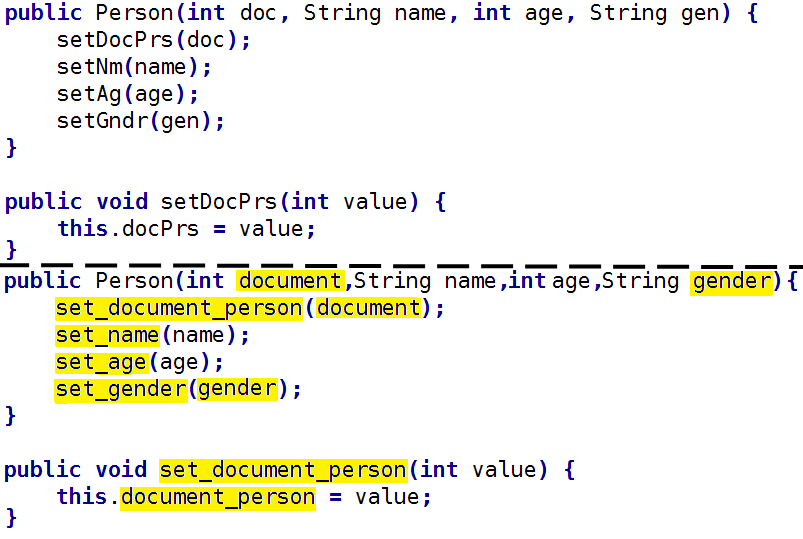
\includegraphics[scale= 0.52]{./cap5/cod.png}
}
\caption{Comparación de un código, antes y después de expandir los ids.}
\label{cod}
\end{figure}

\subsection{Generar un Archivo de Salida con Identificadores Expandidos}

Para ubicarse en el contexto de esta mejora, IDA tiene un panel (Panel de Elementos Capturados) en donde se muestra el código del archivo ingresado para que el usuario lo visualice. 

%Este código se resalta los id con color, cuando se seleccionaba un id en la tabla correspondiente (también lo hace con los comentarios y los literales, ver capítulo 4 para más detalles).

Una propuesta de mejora en la herramienta IDA, consiste en traducir los ids que se muestran en este código.
Esta traducción implica reemplazar cada id ubicado en el código por la expansión que fue llevada a cabo, dado que hay dos tipos de expansiones por cada id (expansión desde Greedy/Samurai), lo que se permitirá es que el usuario pueda elegir entre ambas alternativas la que mejor le parezca. De esta forma, se obtendrá un código más legible y ayudará a comprenderlo más fácilmente. En la figura \ref{cod} se explaya esta idea, aquí se compara un código, antes y después de expandir los ids.

Luego el nuevo código con los ids expandidos se podrá guardar en un nuevo archivo de salida JAVA, este nuevo archivo será funcionalmente equivalente al archivo ingresado, pero tendrá los ids expandidos. Esta idea de traducción y creación de un nuevo archivo, fue tomada de una de las características que posee la herramienta Identifier Restructuring Tool cuyos autores son Tonella y Caprile (ver capitulo 3 sección \ref{sec:algRest}), ya que esta herramienta realiza una traducción similar de ids generando un código más comprensivo.

\subsection{Acoplar a entornos de desarrollos}

Una interesante extensión futura para la herramienta IDA, consiste en adaptarla como extensión (plugin) para un entorno de desarrollo integrado, como es el caso de NetBeans o Eclipse. Esto permitiría que el usuario abra un proyecto JAVA desde estos entornos, e inmediatamente con IDA expanda los ids para mejorar la comprensión. Esta propuesta, en parte es similar a una de la características de la herramienta Identifier Dictionary (IDD), que fue desarrollada por Deissenboeck y Pizka (ver capítulo 3 sección \ref{sec:algIdDic}). La herramienta IDD es un plugin de eclipse que al compilar un proyecto en JAVA, automáticamente captura y enumera dentro de una tabla los ids presentes en el proyecto, luego el usuario puede renombrar cada id desde esta tabla a una forma más comprensiva.

Para la herramienta IDA se propone construir un plugin similar al de IDD, en donde se enumeran los ids en una tabla, pero el renombre de ids en IDA a diferencia de IDD es más automático, ya que IDA expande los ids por medio de las estrategias que tiene implementadas. El usuario solo deberá intervenir para determinar que expansión es la más adecuada, entre los distintos resultados que se obtengan, producto de las diferentes estrategias de análisis de ids ejecutadas.


